
\documentclass[10pt,a4paper,final]{article} %draft

\usepackage[english, russian]{babel}

\usepackage[final]{pdfpages}

\usepackage{textcomp,enumitem}

\usepackage{amsmath,amsthm,amssymb}

\usepackage{listings}
\usepackage{xcolor}
\usepackage{caption}

\definecolor{codegray}{rgb}{0.95,0.95,0.95}
\definecolor{codepurple}{rgb}{0.58,0,0.82}

\lstset{
	extendedchars=true,
	literate=
	{а}{{\selectfont\char224}}1
	{б}{{\selectfont\char225}}1
	{в}{{\selectfont\char226}}1
	{г}{{\selectfont\char227}}1
	{д}{{\selectfont\char228}}1
	{е}{{\selectfont\char229}}1
	{ж}{{\selectfont\char230}}1
	{з}{{\selectfont\char231}}1
	{и}{{\selectfont\char232}}1
	{й}{{\selectfont\char233}}1
	{к}{{\selectfont\char234}}1
	{л}{{\selectfont\char235}}1
	{м}{{\selectfont\char236}}1
	{н}{{\selectfont\char237}}1
	{о}{{\selectfont\char238}}1
	{п}{{\selectfont\char239}}1
	{р}{{\selectfont\char240}}1
	{с}{{\selectfont\char241}}1
	{т}{{\selectfont\char242}}1
	{у}{{\selectfont\char243}}1
	{ф}{{\selectfont\char244}}1
	{х}{{\selectfont\char245}}1
	{ц}{{\selectfont\char246}}1
	{ч}{{\selectfont\char247}}1
	{ш}{{\selectfont\char248}}1
	{щ}{{\selectfont\char249}}1
	{ъ}{{\selectfont\char250}}1
	{ы}{{\selectfont\char251}}1
	{ь}{{\selectfont\char252}}1
	{э}{{\selectfont\char253}}1
	{ю}{{\selectfont\char254}}1
	{я}{{\selectfont\char255}}1
	{А}{{\selectfont\char192}}1
	{Б}{{\selectfont\char193}}1
	{В}{{\selectfont\char194}}1
	{Г}{{\selectfont\char195}}1
	{Д}{{\selectfont\char196}}1
	{Е}{{\selectfont\char197}}1
	{Ж}{{\selectfont\char198}}1
	{З}{{\selectfont\char199}}1
	{И}{{\selectfont\char200}}1
	{Й}{{\selectfont\char201}}1
	{К}{{\selectfont\char202}}1
	{Л}{{\selectfont\char203}}1
	{М}{{\selectfont\char204}}1
	{Н}{{\selectfont\char205}}1
	{О}{{\selectfont\char206}}1
	{П}{{\selectfont\char207}}1
	{Р}{{\selectfont\char208}}1
	{С}{{\selectfont\char209}}1
	{Т}{{\selectfont\char210}}1
	{У}{{\selectfont\char211}}1
	{Ф}{{\selectfont\char212}}1
	{Х}{{\selectfont\char213}}1
	{Ц}{{\selectfont\char214}}1
	{Ч}{{\selectfont\char215}}1
	{Ш}{{\selectfont\char216}}1
	{Щ}{{\selectfont\char217}}1
	{Ъ}{{\selectfont\char218}}1
	{Ы}{{\selectfont\char219}}1
	{Ь}{{\selectfont\char220}}1
	{Э}{{\selectfont\char221}}1
	{Ю}{{\selectfont\char222}}1
	{Я}{{\selectfont\char223}}1,
	numbers=left,
	stepnumber=1,
	firstnumber=1,
	numberstyle=\tiny,
	basicstyle=\ttfamily\footnotesize,
	breakatwhitespace=false,
	breaklines=true,
	captionpos=b,
	keepspaces=true,
	showspaces=false,
	showstringspaces=false,
	showtabs=false,
	tabsize=2,
	frame=single,
	backgroundcolor=\color{codegray},
	commentstyle=\color{codepurple},
}
%\usepackage{fancyvrb}

%\usepackage{fancyhdr}

\usepackage{upgreek}

\usepackage{tipa}

\usepackage{tikz}

\usepackage{graphicx}

\usepackage{pgfplots}

\usepackage{indentfirst}

\usepackage{gensymb}

\usepackage{amssymb}

%\usepackage{pdfpages}

\usepackage[unicode, pdftex, colorlinks, urlcolor=blue]{hyperref}

\usepackage[T2A]{fontenc}

%\usepackage[utf8]{inputenc}

\usepackage[left=2cm,right=2cm,top=2cm,bottom=2cm,bindingo ffset=0cm]{geometry}

\usepackage{graphics}

\linespread{1.5}

\pagestyle{plain}

\usepackage{listings} 
\usepackage{moreverb} 

\setlist[enumerate,itemize]{leftmargin=1.2cm} %отступ в перечислениях

\hypersetup{colorlinks,
	allcolors=[RGB]{0 0 0}}

\lstloadlanguages{ [LaTeX] TeX}

\lstloadlanguages{ [LaTeX] TeX}

\lstset{language =[LaTeX] TeX, 
	extendedchars=true , 
	escapechar = | , 
	frame=tb , 
	commentstyle=\itshape , 
	stringstyle =\bfseries}

\textheight=24cm 
\textwidth=16cm
\oddsidemargin=0pt 
\topmargin=-1.5cm
\parindent=24pt 
\parskip=0pt 
\tolerance=2000 
\flushbottom 

%\usepackage[font=scriptsize]{caption}
\usepackage[labelsep=period]{caption}


\begin{document}
	
	\thispagestyle{empty}
	
	\begin{center}
		{\Large МИНОБРНАУКИ РОССИИ}\\
		~\\
		{\large ФЕДЕРАЛЬНОЕ ГОСУДАРСТВЕННОЕ БЮДЖЕТНОЕ ОБРАЗОВАТЕЛЬНОЕ УЧРЕЖДЕНИЕ ВЫСШЕГО ПРОФЕССИОНАЛЬНОГО ОБРАЗОВАНИЯ}\\
		~\\
		{\Large \bf <<САНКТ-ПЕТЕРБУРГСКИЙ ПОЛИТЕХНИЧЕСКИЙ УНИВЕРСИТЕТ ПЕТРА ВЕЛИКОГО>>}\\
		~\\
		{\large Институт Компьютерных наук и кибербезопасности}\\
		{\large Высшая школа технологий искусственного интеллекта}\\
		{\large Направление 02.03.01 Математика и компьютерные науки}\\
		~\\
		~\\
		~\\
		{\Large \bf Отчет по лабораторной работе №1}\\
	%	{\large {"Программирование и алгоритмизация" \,} }\\
		~\\
		{\Large \bf Реализация двоичного кода Грея, мультимножеств на его основе и операций над мультимножествам}\\
	%	{\Large \bf }\\
		~\\
		~\\
		~\\
		~\\
		~\\
		~\\
		~\\
		~\\
		{\large Обучающийся: \underline{\hspace{3.5cm}} \qquad\qquad Гладков И.А.}\\
		~\\
		{\large Руководитель: \underline{\hspace{3.5cm}} \hspace{14mm} Востров А.В.}\\
		~\\
		~\\
		~\\
	\end{center}
	\begin{flushright}
	
	«\underline{\hspace{1cm}}»\underline{\hspace{3cm}}20\underline{\hspace{0.7cm}}г.
\end{flushright}
~\\
~\\
\begin{center}
	{\large Санкт-Петербург, 2024}
\end{center}
	\newpage

\tableofcontents

\newpage
\section* {Введение}
\addcontentsline{toc}{section}{Введение}
\par Задача лабораторной работы заключается в реализации программы, генерирующей код Грея для заполнения универсума разрядностью, заданной пользователем. На основе универсума создаются два мультимножества А и В. Их заполнение производится либо автомотически, либо вручную, в зависимомости от выбора пользователя. Мощность множеств задает пользователь. Как итог на экран выводятся универсум, множества А и В, а также возможность произвести операции на данными множествами:  объединение, пересечение, разность, арифметическая разность, дополнение, симметрическая разность, арифметическая сумма и арифметическое произведение.
\par Лабораторная работа реализована на языке С++, в среде разработки Visual Studio 2022.

\newpage
\section {Математическое описание}
\subsection {Множество}
\par Множество -- это математический объект, представляющий собой совокупность уникальных элементов, неупорядоченных между собой. Элементы множества могут быть числами, буквами, символами или любыми другими объектами. В математике множества часто обозначают заглавными буквами, например, A или B.
\par Множество может быть пустым, обозначается $\varnothing$. Так же существует
универсум, множество, содержащее все объекты и все множества. Обозначает
U. Пример множества: A = \{3, 6, 1, 7, 4\}


\subsection {Мультимножество}

\par Пусть $\tilde{X}=\langle a_1(x_1),...,a_n(x_n) \rangle$ -- мультимножество над множество $X=\{x_1,...,x_n\}$. Тогда число $a_i$ называется \textit{показателем} элемента $x_i$, множество X -- \textit{носителем} мультимножества $\tilde{X}$, число $m=a_1+ ...+a_n$ -- \textit{мощность} мультимножества $\tilde{X}$, а множество $\tilde{\underline{X}} = \{x_i \in X | a_i>0 \}$ называется \textit{составом} мультимножества $\tilde{X}$.\\
\textbf{Пример} Пусть $\tilde{X}= [a^0b^3c^4]$ --мультимножество над множеством $X=\{a,b,c\}$. Тогда $\tilde{\underline{X}}= \{b,c\}$.

Мультимножество  $\tilde{X}=\langle a_1(x_1),...,a_n(x_n)\rangle$ над множеством $X=\{x_1,...,x_n\}$ называется \textit{индикатором}, если $\forall i \in 1..n (a_i =0 \lor a_i =1)$.\\
\textbf{Пример} Мультимножество $\tilde{X}=\langle b;c \rangle$ является индикатором над множеством $X=\{a,b,c\}$, причем $\tilde{\underline{X}}=\{b,c\}$.

\par Над мультимножествами определены следующие операции:  объединение, пересечение, разность, арифметическая разность, дополнение, симметрическая разность, арифметическая сумма, арифметическое произведение.

\begin{quote}
$\circ$ Для двух мультимножеств A и B, \textit{\underline{пересечение}} (А $\cap$ В) будет мультимножеством, содержащим элементы, которые присутствуют в обоих мультимножествах, причем кратность каждого элемента в пересечении будет минимумом его кратности в A и B.

$$C=A \cap B =\{k^{min\{m_{i1},m_{i2}\}}: k^{m_{i1}}\in A \land k^{m_{i2}}\in B \}$$


$\circ$ Для двух мультимножеств A и B, \textit{\underline{объединение}} (A $\cup$ B) будет мультимножеством, содержащим все элементы, присутствующие в A и B, и их кратности будут равны максимуму их кратностей в A и B.

$$C=A \cup B =\{k^{max\{m_{i1},m_{i2}\}}: k^{m_{i1}}\in A \lor k^{m_{i2}}\in B \}$$


$\circ$ Для двух мультимножеств A и B, \underline{\textit{разность}} обозначается как 
А\textbackslash В. Результатом этой операции будет мультимножество, содержащее элементы, которые одновременно присутствуют в A и $\overline{B}$, и кратность каждого такого элемента будет равна минимальной кратности мультимножеств A и $\overline{B}$. 

$$ C=A\textbackslash B=A \cap \overline{B}=\{k^{min\{m_{i1},m_{i2}\}} :k^{m_{i1}} \in A \land k^{m_{i2}} \in \overline{B} \}$$


$\circ$ \textit{\underline{Дополнение}} мультимножества относительно универсума представляет собой операцию, в результате которой получается мультимножество, содержащее элементы универсума, не входящие в исходное мультимножество, и их кратности соответствуют кратностям в универсуме.

Дополнение мультимножества A относительно универсума U обозначается как $\overline{\text{А}}$ и содержит элементы, присутствующие в U, но отсутствующие в A, с кратностями, соответствующими кратностям в U, то есть кратность элемнтов будет равна сумме кратностей соответсвубщих элементов в универсуме U и мультимножестве A.

$$\overline{A}=\{k^{m_{iU}-m_{i1}}:k^{m_{i1}} \in A \land k^{m_{iU}} \in U\}$$


$\circ$ \textit{\underline{Симметрическая разность}} мультимножеств A и B обозначается как А$\triangle$В и представляет собой мультимножество, содержащее элементы, которые присутствуют в A или B, но не в обоих одновременно, то есть состоит их тех элементов мультимножества А и В, кратности которых различны. Кратность результирующего множества равно модулю разности кратностей этих элементов в А и В.

$$ C=A \triangle B= \{k^{\left| m_{i1} - m_{i2}\right|}:k^{m_{i1}} \in A \land k^{m_{i2}} \in B \}$$


$\circ$ Для двух мультимножеств A и B, \underline{\textit{арифметическая разность}} обозначается как  А $-$ В . Результатом данной операции является мультимножество, состоящее из элементов мультимножества А, кратность которых превышает кратность этих же элементов в мультимножестве В. Кратность каждого элемента результирующего мультимножества равна разности кратностей элементов мультимножеств А и В. Но разность не может быть меньше нуля.
$$ C= A-B=\{k^{max\{0,m_{i1}-m_{i2}\}}:k^{m_{i1}} \in A \lor k^{m_{i2}} \in B \}$$
 
 
$\circ$ Для двух мультимножеств A и B, \underline{\textit{арифметическая сумма}} обозначается как  А $+$ В. Результатом данной операции является мультимножество, состоящее из всех элементов мультимножеств А и В, кратность каждого элемента равна сумме кратностей в складываемых мультимножествах. Но сумма кратностей не может превышать кратности в универсуме. 
$$ C= A-B=\{k^{min\{m_{i1}+m_{i2},m_{iU}\}}:k^{m_{i1}} \in A \lor k^{m_{i2}} \in B, k^{m_{iU}} \in U \}$$


$\circ$ Для двух мультимножеств A и B, \underline{\textit{арифметическое произведение}} обозначается как  А $*$ В. Результатом данной операции является мультимножество, состоящее из элементов, которые присутствуют в каждом из мультимножеств, и их кратность равна произведению кратностей соответствующих элементов в перемножаемых мультимножествах. Но произведение не может превышать кратности в универсуме.
$$ C= A-B=\{k^{min\{m_{i1}*m_{i2},m_{iU}\}}:k^{m_{i1}} \in A \land k^{m_{i2}} \in B \land k^{m_{iU}} \in U \}$$

\end{quote}
 
\subsection {Бинарный код Грея}
\par Код Грея  представляет собой последовательность двоичных чисел, в которой каждое следующее число отличается от предыдущего всего лишь одним битом. Формируется относительно заданной разрядности при помощи особого алгорима.\\
Пример кода Грея разрядности 2:\\
00, 01, 10, 11

Ниже, в \textbf{листинге 1}, представлен алгоритм, генерурующий последовательность всех подмножеств n-элементного множества, где каждое следующее подмножество получается из предыдущего удалением и добавлением в точности одного элемента. 
Вход: n >= 0 - мощность множества.
Выход: последовательность кодов множества B 

\begin{lstlisting}[caption={Построение бинарного кода Грея}]
	Вход: n >= 0 - мощность множества.
	Выход: последовательность кодов множества B 
	B: array[1..n] of 0..1 {Битовая шкала для представления подмножеств}
	for i from 1 to n do: B[i]:= 0 for {инициализация}
	yeild B{пустое множество}
	for i from 1 to 2^n - 1 do: 
	p:= Q[i] {Определение номера элемента, подлежащего добавлению или удалению}
	B[p]:= 1 - B[p] {Добавление или удаление элемента}
	yeild B {очередное подмножество}
	end for  
	
\end{lstlisting}

\par Ниже, в \textbf{{листинге 2}}, представлена функция, с помощью которой определяется номер разряда, подлежащего изменению, возвращает количество нулей на конце двоичной записи числа i, увеличенное на 1
\par Вход: i - номер подмножества 
\par Выход: номер измеряемого разряда.

\begin{lstlisting}[caption={Функция определения номера измеряемого разряда}]
	Вход: i - номер подмножества
	Выход: номер измеряемого разряда
	q:= 1
	j:= i
	while (j % 2 = 0) do
	j:= j/2
	q:= q + 1
	end while
	return q  
	
\end{lstlisting}

\newpage
\section {Особенности реализации}
\subsection {Класс GrayCode}
\par Класс GrayCode -- основной класс в моей лабораторной работе, он отвечает за универсум и код Грея. Он является базовым классом для класса содержащего мультимножество.

\par Класс содержит переменные:
\begin{quote}
	$\circ$ int \textbf{n} -- разрядность кода Грея
	
	$\circ$ int \textbf{k} -- количесво чисел в коде Грея $k=2^n$
	 
	$\circ$ int \textbf{Count} -- количество различных элементов
	 
	$\circ$ vector <int> \textbf{Codes} -- массив содержаший код Грея
	
	$\circ$ vector <int> \textbf{Krat} -- массив сожержащий кратность каждого элемента кода Грея


\end{quote}

\subsubsection {Конструктор с параметром GrayCode}
\par Вход: кратность универсума.
\par Выход: сформированный универсум.
\par Переменной \textbf{n} присваивается значение передваемой переменной \textit{\textbf{а}}, переменная \textbf{k} считается по формуле $k=2^n$ с помощью \textit{for}, \textbf{Codes} увеличивается до размера k $\times$ n с помощью метода \textit{resize} (далее будет понятно почему). После создается код Грея по созданному мною алгориму:\\
(Напишем элементы кода Грея разрядности 3 друг под другом)\\
000\\
001\\
010\\
011\\
100\\
101\\
110\\
111\\

Если посмотреть на каждый столбец (их всего 3 в данном случае), заметим что в первом "0" сменяется на "1" (а также "0" на "1" в дальнейшем) через \textbf{k}/2, то есть 8/2=4, во втором в два раза чаще, то есть через 4/2=2 числа, и так далее. для этого создается переменная \textbf{buf} = \textbf{k}/2, который будет использоваться и зменяться в алгоритме. При помощи этой перемнной и нескольких проверок в \textit{for} будет ставится либо "0", либо "1". Также все эти столбцы записываются попорядку в \textbf{Codes}, то есть "000011110011001101010101" для этого нужно было создать массив размером  k $\times$ n.
\par Потом \textbf{Krat} увеличивается с помощью метода \textit{resize} до размера \textbf{k}. Затем туда записывается случайное значение кратности для каждого элемента в коде Грея. Код конструктора представлен в \textbf{листинге 3}, ниже.
	
	

	
\begin{lstlisting}[caption={Конструктор GrayCode}]
	GrayCode::GrayCode(int a) {
		n = a;
		if (a == 0)
		k = 0;
		else
		k = 2;
		for (int i = 0; i < n - 1; i++) {
			k *= 2;
		}
		Count = k;
		Codes.resize(k * n);        
		int buf = k / 2;
		for (int m= 0; m < n; m++) {
			static int i = 0;
			static int p = 1;
			int f = 0;
			for (i; i < k * p; i++) {
				if (f < buf)
				Codes[i] = 0;
				else
				Codes[i] = 1;
				f++;
				if (f == buf * 2)
				f = 0;
			}
			buf = buf / 2;
			p++;
		} 
		Krat.resize(k);
		srand(time(0));
		max = 0;
		for (int i = 0; i < k; i++) {
			Krat[i] = rand() % 99 + 1 ;
			max += Krat[i];
		}       
	}
\end{lstlisting}

	
\subsubsection {Методы Getk, Getn, GetCodes, GetKrat, Print}

\par Метод \textit{Getk}, возвращает значение переменной \textbf{k}, то есть количесво чисел в коде Грея $k=2^n$. Этот метод необходим в формировании мультимножества: используется в циклах for, чтоб не было выхода за границы массива.
\par Вход: получение количества чисел в коде Грея.
\par Выход: количесво чисел в коде Грея.\\

\begin{lstlisting}[caption={Метод Getk}]
int GrayCode::Getk() {
	return k;
}
\end{lstlisting}



\par Метод \textit{ Getn()} возвращает значение переменной \textbf{n}, то есть разрядность кода Грея. Используется также при формировании мультимножеств: когда у пользователя спрашивают какого кратности будет то или иное число, которое показывается в строке припомощи данного метода.
\par Вход: получение разрядности кода Грея.
\par Выход: разрядность кода Грея.

\begin{lstlisting}[caption={Метод Getn}]
int GrayCode::Getn() {
	return n;
}
\end{lstlisting}



\par Метод \textit{ GetCodes()} возвращает массив \textbf{Codes}, содержащий код Грея. Необходим в формировании мультимножеств, так как класс Multi не создает заного код Грея, а берет их класса GrayCode.
\par Вход: получение массива, содержащего код Грея.
\par Выход: массив, содержащий код Грея.

\begin{lstlisting}[caption={Метод GetCodes}]
vector <int> GrayCode::GetCodes() {
	return Codes;
}
\end{lstlisting}




\par Метод \textit{ GetKrat()} массив \textbf{Krat}, содержащий крастность элементов в универсуме. Необходим при создании мультимножеств, для корректного заполнения. В мульти множестве кратность элемента не должна превышать кратности в универсуме. Метод используется для проверок данного правила. 
\par Вход: получение массива, содержащего кратность элементов в универсуме.
\par Выход: массив, содержащий крастность элементов в универсуме.

\begin{lstlisting}[caption={Метод GetKrat}]
vector <int> GrayCode::GetKrat() {
	return Krat;
}
\end{lstlisting}



\par Метод \textit{ Print()} Выводит на экран универсум. Так как весь код Грея представлен в одном массиве, необходимо проходить по массиву с определенным шагом и выводить по одному символу.
\par Вход: намерение увидеть универсум на консоли 
\par Выход: печать универсума на консоль 

\begin{lstlisting}[caption={Метод Print}]
	void GrayCode::Print() {
		cout << "\n  УНИВЕРСУМ\n\n";
		
		if (n == 0) {
			printf("Пуст..\n");
		}
		else {
			for (int i = 0; i < k; i++) {
				if (Krat[i] != 0) {
					cout << "   ";
					for (int j = 0; j < k * n; j += k) {
						cout << "  " << Codes[i + j];
					}
					
					cout << "  [" << i << "]" << " :  " << Krat[i] << "\n";
				}
			}
		}
	}
\end{lstlisting}


\newpage
\subsection {Класс Multi}

\par Класс Multi отвечает за мультимножества. Данный класс наследник от класса GrayCode. В нем создается мультимножество на основе универсума. Экземпляры данного класса будут различными мультимножествами, то есть один экземпляр отвечает за одно мультимножество. Он содержит переменные:
\begin{quote}
%	$\circ$ int \textbf{m} -- мощность данного мультимножества
	
	$\circ$ int \textbf{Count} -- количесво различных элементов в мультимножестве
	
	$\circ$ vector <int> \textbf{elems} -- массив содержаший кратность для каждого числа 
	
	$\circ$ GrayCode* \textbf{base} -- указатель на экземпляр класса GrayCode содержащий универсум
	
	$\circ$ vector<bool \textbf{Show} -- массив флагов, показывающие, выбран ли тот или иной элемент универсума в мультимножестве.
	
\end{quote}

\subsubsection {Конструктор с параметрами Multi}
\par Вход: Количество различных элементов, указатель на экземпляр класса с универсумом и переменная, показывающая, будет ли этот экземпляр класса входным мультимножеством или резельтатом операций над входными мультимножествами.
\par Выход: Заготовка для формирования универсума.
\par Переменной \textbf{Count} присваивается передаваемое значение \textit{а}, то есть мощность мультимножества. Далее указателю \textbf{base} присваивается адресс экземпляра класса GrayCode. После массив \textbf{elems} увеличивается до размера количества различных чисел в универсуме. Кратность каждого равна нулю. Затем пользователь решает, будет он выбирать различные элементы мультимножества в ручную или автоматически. Если пользователь выбирает заполнить вручную, то он вводит по одному элементы, если автоматически, то элементы выбираются случайно. Код конструктора представлен ниже, в \textbf{листинге 10}.

\begin{lstlisting}[caption={Конструктор Multi}]
	Multi::Multi(int a, GrayCode* b, bool flag) {
		Count = a;
		base = b;
		elems.resize(base->Getk(), 0);
		Show.resize(base->Getk(), 0);
		
		if (base->Getk() != 0 && flag) {
			
			regex powerful("^[0-9]{0,50}$");
			
			printf("Хотите ли вы конкретные ненулевые значения - [1], или же их выбрать автоматически - [0]?\n");
			string s;
			while (true) {
				cin >> s;
				if (s == "0" or s == "1")
				break;
				else printf("\nВведите либо [1] либо [0]\n");
			}
			if (stoi(s) == 1) {
				printf("\nВводите по одному элементы\n");
				for (int i = 0; i < Count; i++) {
					cin >> s;
					if (regex_match(s, powerful) && stoi(s) >= 0 && stoi(s) < this->base->Getk()) {
						if (Show[stoi(s)] == 1) {
							printf("Ну зачем же вы пишете повторяющийся элемент?\n");
							i--;
						}
						else
						Show[stoi(s)] = 1;
					}
					else {
						std::cout << "Ошибка ввода!\n";
						i--;
						
					}
				}
			}
			else {
				srand(time(0));
				for (int i = 0; i < Count; i++) {
					int r = rand() % base->Getk();
					if (Show[r] == 1)
					i--;
					else {
						Show[r] = 1;
					}
				}
			}
		}
	}
\end{lstlisting}

\subsubsection {Методы Avto(), Hand(), Print(string s)}
\begin{quote}
	$\circ$ Метод \textit{Avto()} заполняет массив\textbf{elems} случайными кратностостями элементы мультимножества. Проходится по массиву, заполняя значения кратности рандомно, при этом проводится проверка, чтобы кратность была не больше чем в универсуме. 
	\par Вход: намерение сформировать мультимножество автоматически.
	\par Выход: сформированное мультимножество.
	
	\begin{lstlisting}[caption={Метод Avto}]
		void Multi::Avto() {
			srand(time(0));
			for (int i = 0; i < base->Getk(); i++) {
				if (Show[i] != 0) {
					int r = rand() % base->GetKrat()[i];
					elems[i] = r;
				}
			}
		}
	\end{lstlisting}
	
	
	$\circ$ Метод \textit{Hand()} заполняет массив \textbf{elems} кратностями элементов, вводимыми с консоли, пользователем. В цикле каждый раз у пользователя спрашивают какая кратность будут у того или иного числа, и производится проверка на корректность пользовательского ввода и на то, чтобы вводимая кратность не превышала кратности в универсуме.
	\par Вход: намерение  сформировать мультимножество пользовательским вводом
	\par Выход: сформированное мультимножество
	
	\begin{lstlisting}[caption={Метод Hand}]
		void Multi::Hand() {
			
			cout << "\n-----------------------------------";
			cout << "\nВы решили заполнить массив вручную\n\n";
			
			srand(time(0));
			
			for (int i = 0; i < base->Getk(); i++) {
				if (Show[i] != 0) {
					cout << "Какая кратность будет у этого числа? ";
					for (int j = 0; j < base->Getn(); j++) {
						cout << base->GetCodes()[i + j * base->Getk()]  ;
					}
					cout <<" ["<<i<<"]: "<< base->GetKrat()[i]<<"\n";
					string bit;
					regex powerful("^[0-9]{0,50}$");
					while (true) {
						cin >> bit;
						if (regex_match(bit, powerful) && stoi(bit) >= 0 && stoi(bit) <= this->base->GetKrat()[i]) {
							break; // Ввод соответствует регулярному выражению, выходим из цикла
						}
						else {
							std::cout << "Ошибка ввода!\n";
						}
					}
					elems[i] = stoi(bit);
				}
			}
	\end{lstlisting}
	
	
	$\circ$ Метод \textit{Print(string s)} выводит на экран мультимножество и название \textit{string s}, которое вводится в параметрах метода. Вывод на экран аналогичный универсуму, только перед ним пишется название универсума.
	\par Вход: название мультимножества
	\par Выход: вывод в консоль мультимножество с его названием.
	 
	\begin{lstlisting}[caption={Конструктор Print}]
		void Multi::Print(string s) {
			printf("\n||||||||||||||||||||||||||||||||");
			cout << "\n    "<<s<<"\n\n";
			bool flag = 1;
			for (int i = 0; i < base->Getk(); i++) {
				if (Show[i] != 0) {
					cout << "   ";
					for (int j = 0; j < base->Getk() * base->Getn(); j += base->Getk()) {
						cout << "  " << (base->GetCodes().at(i+j));
						flag = 0;
					}
					
					cout << "  [" << i << "]"<< " :  " << elems[i] << "\n";
				}
			}
			if (flag)
			printf("Пустое множество\n");
			printf("\n||||||||||||||||||||||||||||||||\n");
	\end{lstlisting}
	
\end{quote}

\subsubsection {Метод Unification -- объединение мультимножеств А и В}
\par Вход: ссылка на мультимножество А и ссылка на мультимноество В. 
\par Выход: результат операции объединения мультимножеств А и В.
\par Функция выполняет операцию объединения двух мультимножеств \textit{А} и \textit{В}, то есть находит максимум из двух кратностей одинаковых элементов в двух мультимножествах передаваемых через параметры функции. Максимальная кратность элемента записывается в \textbf{this->elems[i]}, то есть в экземпляр класса, в котором выполняется данный метод.

\begin{lstlisting}[caption={Метод Unification}]
	void Multi::Unification(Multi& a, Multi& b) { //объединение
		for (int i = 0; i < base->Getk(); i++) {
			this->elems[i] = a.elems[i] > b.elems[i] ? a.elems[i] : b.elems[i];
			if (elems[i] != 0)
			Show[i] = 1;
		}
	}
	\end{lstlisting}
	

\subsubsection {Метод Intersection -- пересечение мультимножеств А и В}
\par Вход: ссылка на мультимножество А и ссылка на мультимноество В. 
\par Выход: результат операции пересечения мультимножеств А и В.
\par Функция выполняет операцию пересечения двух мультимножеств \textit{А} и \textit{В}, то есть находит минимум из двух кратностей одинаковых элементов в двух мультимножествах пераваемых через параметры функции. Минимальная кратность элемента записывается в \textbf{this->elems[i]}, то есть в экземпляр класса, в которм выполняется данный метод.

\begin{lstlisting}[caption={Метод Intersection}]
	void Multi::Intersection(Multi& a, Multi& b) { //Пересечение 
		for (int i = 0; i < base->Getk(); i++) {
			this->elems[i] = a.elems[i] < b.elems[i] ? a.elems[i] : b.elems[i];
			if (elems[i] != 0)
			Show[i] = 1;
		}
	}
\end{lstlisting}


\subsubsection {Метод DifferenceA -- разность мультимножеств А и В}
\par Вход: ссылка на мультимножество А и ссылка на мультимноество В. 
\par Выход: результат операции разности мультимножеств А и В.
\par Функция выполняет операцию разности двух мультимножеств \textit{А} и \textit{В} (A\textbackslash B = $A \cap \overline{B})$, то есть определяет минимальную кратность соответствующих элементов в мультимножествах А и $\overline{B}$, и записывает результат в результирующее мультимножество.

\begin{lstlisting}[caption={Метод DifferenceA}]
	void Multi::DifferenceA(Multi& a, Multi& b){ // разность множеств A и B
		for (int i = 0; i < base->Getk(); i++) {
			this->elems[i] = a.elems[i] < (base->GetKrat()[i]-b.elems[i]) ? a.elems[i] : base->GetKrat()[i] - b.elems[i];
			if (elems[i] != 0)
			Show[i] = 1;
		}
	}
\end{lstlisting}


\subsubsection {Метод DifferenceB --  разность мультимножеств B и A}
\par Вход: ссылка на мультимножество А и ссылка на мультимноество В. 
\par Выход: результат операции разности мультимножеств В и А.
\par Функция выполняет операцию разности двух мультимножеств \textit{В} и \textit{А} (В\textbackslash А = $В \cap \overline{А})$, то есть определяет минимальную кратность соответствующих элементов в мультимножествах В и $\overline{А}$, и записывает результат в результирующее мультимножество.

%\par Функция определяет арифметическую разность двух мультимножеств \textit{b} и \textit{a} (B \textbackslash A), то есть находит кратность элементов, находящихся в мультимножестве \textit{b}, и не находящихся в \textit{a}. То есть из кратности элемента мультимножества \textit{b} вычитает кратность эелемента мультимножества \textit{a}, если кратность в \textit{a} больше чем в \textit{b}, то итоговая кратность будет равна нулю.

\begin{lstlisting}[caption={Метод DifferenceB}]
	void Multi::DifferenceB(Multi& a, Multi& b){ //разность множеств B и A
		for (int i = 0; i < base->Getk(); i++) {
			this->elems[i] = (base->GetKrat()[i]-a.elems[i]) < b.elems[i] ?base->GetKrat()[i]- a.elems[i] : b.elems[i];;
			if (elems[i] != 0)
			Show[i] = 1;
		}
	}
\end{lstlisting}


\subsubsection {Метод AdditionA -- дополнение мультимножества А}
\par Вход: ссылка на мультимножество А и ссылка на мультимноество В. 
\par Выход: результат операции дополнения мультимножества А.
\par Функция выполняет операцию дополнения мультимножества \textit{А}, то есть находит разности кратностей элементов в универсуме и в мультимножестве \textit{А}.

\begin{lstlisting}[caption={Метод AdditionA}]
	void Multi::AdditionA(Multi& a, Multi& b){ //Дополнение множества A
		for (int i = 0; i < base->Getk(); i++) {
			this->elems[i] =  a.base->GetKrat().at(i)-a.elems[i]>0 ? a.base->GetKrat()[i] - a.elems[i] : 0;
			if (elems[i] != 0)
			Show[i] = 1;
		}
	}
\end{lstlisting}


\subsubsection {Метод AdditionB -- дополнение мультимножества В}
\par Вход: ссылка на мультимножество А и ссылка на мультимноество В. 
\par Выход: результат операции дополнения мультимножества В.
\par Функция выполняет операцию дополнения мультимножества \textit{В}, то есть находит разности кратности элементов в универсуме и в мультимножестве \textit{В}.

\begin{lstlisting}[caption={Метод AdditionB}]
	void Multi::AdditionB(Multi& a, Multi& b) { //Дополнение множества B
		for (int i = 0; i < base->Getk(); i++) {
			this->elems[i] = b.base->GetKrat().at(i) - b.elems[i] > 0 ? b.base->GetKrat()[i] - b.elems[i] : 0;
			if (elems[i] != 0)
			Show[i] = 1;
		}
	}
\end{lstlisting}


\subsubsection {Метод Sim\_Difference -- симметрическая разность мультимножеств А и В}
\par Вход: ссылка на мультимножество А и ссылка на мультимноество В. 
\par Выход: результат операции симметрической разности мультимножеств А и В.
\par Функция выполняет операцию симметрической разности двух мультимножеств \textit{А} и \textit{В} (A\textbackslash B), то есть находит кратность элементов, находящихся либо в мультимножестве \textit{А}, либо в мультимножестве \textit{В}, но не находящихся одновременно в \textit{А} и \textit{В}. То есть если кратность в \textit{А} больше кратности в \textit{В}, то выполняется разность кратностей из \textit{А} и \textit{В}, и если кратность в \textit{В} больше кратности в \textit{А}, то выполняется разность кратностей \textit{В} и \textit{А}, а иначе кратность равна нулю.
 
 \begin{lstlisting}[caption={Метод Sim\_Difference}]
 	void Multi::Sim_Difference(Multi& a, Multi& b){ //Симметрическая разность множеств A и B
 		for (int i = 0; i < base->Getk(); i++) {
 			this->elems[i] = a.elems[i] - b.elems[i] > 0 || b.elems[i] - a.elems[i] > 0 ? 
 			(a.elems[i] - b.elems[i] > 0? a.elems[i] - b.elems[i] : b.elems[i] - a.elems[i] ): 0;
 			if (elems[i] != 0)
 			Show[i] = 1;
 		}
 	}
 \end{lstlisting}
 
 
 \subsubsection {Метод Ar\_DifferenceA -- арифметическая разность мультимножеств А и В}
\par Вход: ссылка на мультимножество А и ссылка на мультимноество В. 
 \par Выход: результат операции арифметической разности мультимножеств А и В.
\par Функция выполняет операцию арифметической разности мультимножеств \textit{А} и \textit{В}. Производится разность кратности элемента мультимножества \textit{А} и мультимножества \textit{В}. Итог записывается в результирующее мультимножество, но если разность получается отрицательная, то записывается ноль.
 \begin{lstlisting}[caption={Метод Ar\_DifferenceA}]
 	void Multi::Ar_DifferenceA(Multi& a, Multi& b) { //Арифметическая разность множеств A и B
 		for (int i = 0; i < base->Getk(); i++) {
 			this->elems[i] = a.elems[i] - b.elems[i] > 0 ? a.elems[i] - b.elems[i] : 0;
 			if (elems[i] != 0)
 			Show[i] = 1;
 		}
 	}
 \end{lstlisting}
 
 
 \subsubsection {Метод Ar\_DifferenceB -- арифметическая  разность мультимножеств В и А}
\par Вход: ссылка на мультимножество А и ссылка на мультимноество В. 
 \par Выход: результат операции арифметической разности мультимножеств В и А.
 \par Функция выполняет операцию арифметической разности мультимножеств \textit{В} и \textit{А}. Производится разность кратности элемента мультимножества \textit{В} и мультимножества \textit{А}. Итог записывается в результирующее мультимножество, но если разность получается отрицательная, то записывается ноль.
 \begin{lstlisting}[caption={Метод Ar\_DifferenceB}]
 	void Multi::Ar_DifferenceB(Multi& a, Multi& b) { //Арифметическая разность множеств B и A
 		for (int i = 0; i < base->Getk(); i++) {
 			this->elems[i] = b.elems[i] - a.elems[i] > 0 ? b.elems[i] - a.elems[i] : 0;
 			if (elems[i] != 0)
 			Show[i] = 1;
 		}
 	}
 \end{lstlisting}
 

\subsubsection {Метод Ar\_Summ -- арифметическая  сумма мультимножеств А и В}
\par Вход: ссылка на мультимножество А и ссылка на мультимноество В. 
 \par Выход: результат операции арифметической суммы мультимножеств А и В.
\par Функция выполняет операцию арифметической разности мультимножеств \textit{А} и \textit{В}. Производится сумма кратности элемента мультимножества \textit{А} и мультимножества \textit{В}. Итог записывается в результирующее мультимножество, но если сумма получается больше кратности в универсуме, то записывается кратность элемента универсума.
\begin{lstlisting}[caption={Метод Ar\_Summ}]
	void Multi::Ar_Summ(Multi & a, Multi & b){//арифметическая сумма А и В
		for (int i = 0; i < base->Getk(); i++) {
			this->elems[i] = b.elems[i] + a.elems[i] < base->GetKrat()[i] ? b.elems[i] + a.elems[i] : base->GetKrat()[i];
			if (elems[i] != 0)
			Show[i] = 1;
		}
	}
\end{lstlisting}


 \subsubsection {Метод Ar\_Prod -- арифметическое произведение мультимножеств А и В}
\par Вход: ссылка на мультимножество А и ссылка на мультимноество В. 
 \par Выход: результат операции арифметического произведения мультимножеств А и В.
\par Функция выполняет операцию арифметического произведения мультимножеств \textit{А} и \textit{В}. Производится произведение кратности элемента мультимножества \textit{А} и мультимножества \textit{В}. Итог записывается в результирующее мультимножество, но если произведение получается больше кратности в универсуме, то записывается кратность элемента универсума.
\begin{lstlisting}[caption={Метод Ar\_Prod}]
	void Multi::Ar_Prod(Multi & a, Multi & b){//арифметическое произведенеие А и В
		for (int i = 0; i < base->Getk(); i++) {
			this->elems[i] = b.elems[i] * a.elems[i] < base->GetKrat()[i] ? b.elems[i] * a.elems[i] : base->GetKrat()[i];
		}
	}
\end{lstlisting}


 
\newpage
\subsection{Функция main и проверка на корректность пользовательского ввода}
\par Весь интерфейс вывода на экран прописан в функции \textit{main}, также там используется проверка на корректность при каждом вводе пользователя, чтобы нельзя было ввести несответствующее значение. 
Используются регулярные выражения (regex) бля проверки ввода определенных символов, в данной лабораторной это цифры. Также вместе с регулярными выражениями используется проверка диапазона чисел, изменяющаяся от места запроса ввода данных пользователя. Пример использования в лабораторной ниже, в \textbf{листинге 25}.

\par Вход: желание ограничить пользовательский ввод.
\par Выход: ограничение пользовательского ввода.
\begin{lstlisting}[caption={Пример корректности пользовательского ввода}]
regex powerful("^[0-9]{0,50}$");
//создание универсума
string buf;

cout << "Введите разрядность УНИВЕРСУМА (целое число 0-10)\n";
while (true) {
	cin >> buf;
	if (regex_match(buf, powerful) && stoi(buf) >= 0 && stoi(buf) <= 10) {
		break; // Ввод соответствует регулярному выражению, выходим из цикла
	}
	else {
		std::cout << "\nОшибка ввода! Ведите число от 0 до 10\n\n";
	}
}
int n = stoi(buf);
GrayCode m(n);
\end{lstlisting}

\par В начале у пользователя запрашивается разрядность универсума, после выводится универсум. 
\par Затем предлагается заполнить мультимножество А, вручную или автоматически. Следующим шагом необходимо решить сколько будет уникальных элементов в мультимножестве. Далее предоставляется выбор заполнения этих элементов: вручную, либо автоматически. Пользователь выбирает, и происходит заполнение мультимножества различными элементами. При первом запросе, если было выбрано автоматическое запонение, то кратности к уникальным числам унивесума выбираются автоматически, не превышая кратности в универсуме. Если же было выбрано ручное заполнение, то программа будет запрашивать кратность от пользователя для каждого уникального элемента мультимножества. После на экран выводится сформированное мультимножество А.
\par Аналогичные действия производятся с мультимножеством В.
\par Следующим шагом создается экземпляр класса \textit{Multi}, оно будет являтся результирующим мультимножеством операций между А и В. Затем пользователю предоставляется возможность выполнить различные действия с мультимножествами А и В, а также выйти из программы. В зависимости от пользователя, выполняется тот или иной метод класса \textit{Multi} в экземпляре класса, созданным чуть ранее (результирующее мультимножество).
 
 \section {Результаты работы}
 \par Ниже будут представлены илюстрации, показывающие результат проделанной работы, и то как эту программу видит пользователь. 
 
 Создание универсума разрядности, которую ввел пользователь, изображено на \textit{рисунке 1}.
 
 \begin{figure}[h!]
 	\centering
 	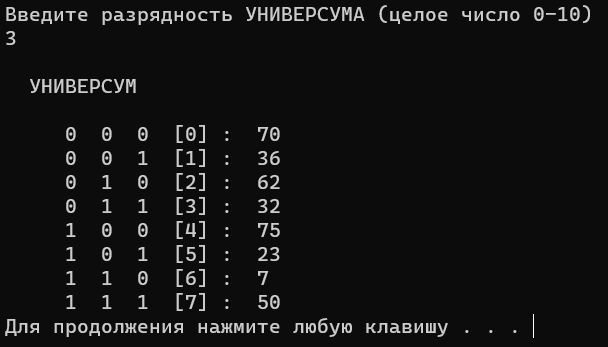
\includegraphics[width=0.8\textwidth]{1}
 	\caption{Создание универсума, заданной пользователем разрядности}
 \end{figure}
 
  Формирование двух мультимножеств изображено на \textit{рисунках 2 - 4}.
  
  Автоматическое заполнение мультимножества А  и автоматический выбор четырех различных ненулевых элементов показано на \textit{рисунке 2}.
 \begin{figure}[h!]
 	\centering
 	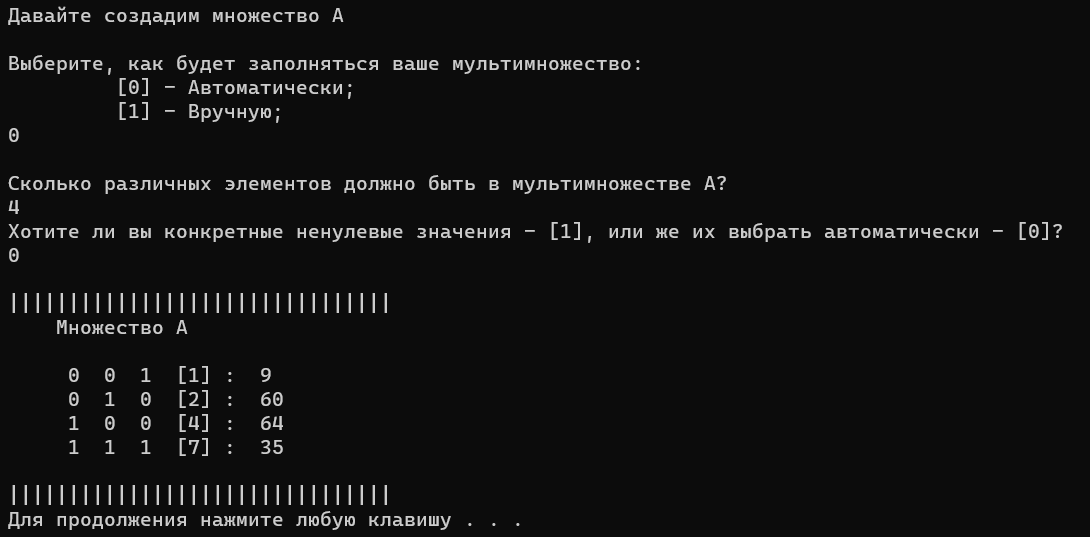
\includegraphics[width=0.85\textwidth]{2}
 	\caption{Автоматическое заполнение мультимножества А  и автоматический выбор четырех различных ненулевых элементов}
 \end{figure}
  \clearpage
%\newpage
Ввод различных ненулевых элементов в мультимножество В вручную и заполнение кратностей выбранных элементов тоже вручную можно увидеть на \textit{рисунках 3-4}

\begin{figure}[h!]
	\centering
	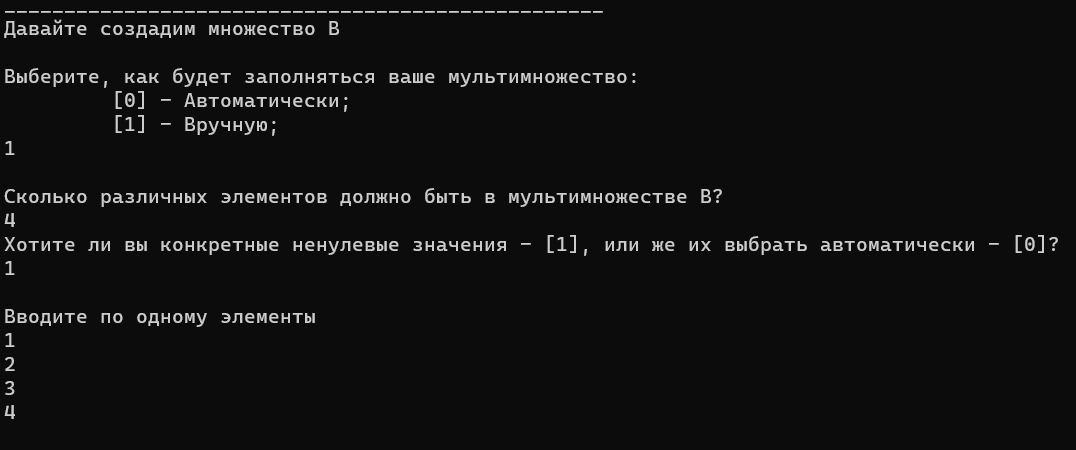
\includegraphics[width=1.1\textwidth]{3}
	\caption{Ввод различных ненулевых элементов в мультимножество В вручную}
	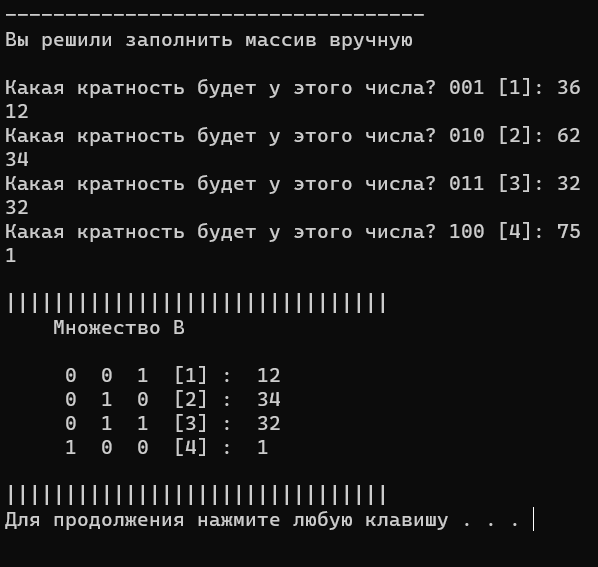
\includegraphics[width=0.8\textwidth]{4}
		\caption{Заполнение кратностей выбранных элементов вручную }
\end{figure}
\clearpage
%\newpage

Меню с возжными операциями над операциями и дополнительные действиями над множествами множествами изображено на \textit{рисунке 5}
\begin{figure}[h!]
	\centering
		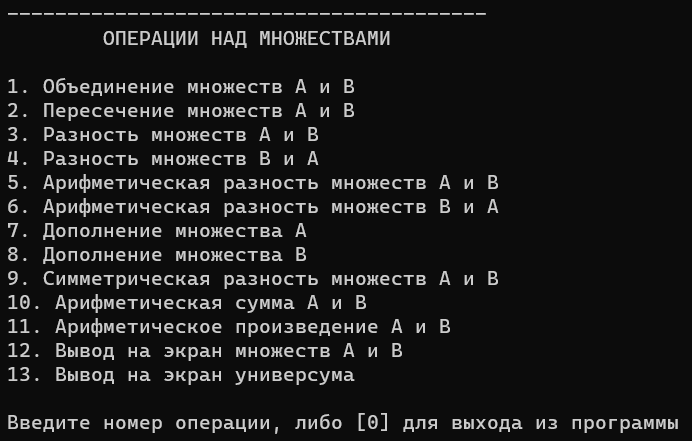
\includegraphics[width=0.8\textwidth]{5}
	\caption{Перечень операций над мультимножествами А и В}
\end{figure}

		Все операции над множествами, реализованные в лабораторной работе, а также дополнительные действия показаны на рисунках 6-17
	
	\begin{figure}[h!]
		\centering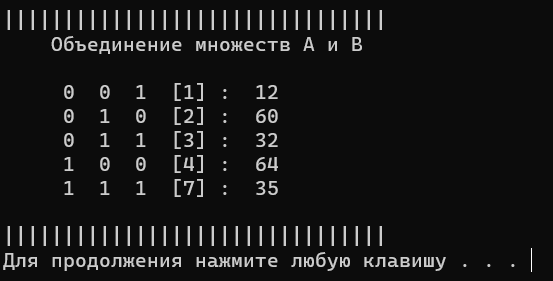
\includegraphics[width=0.6\textwidth]{6}
	\caption{Объединение мультимножеств А и В}
		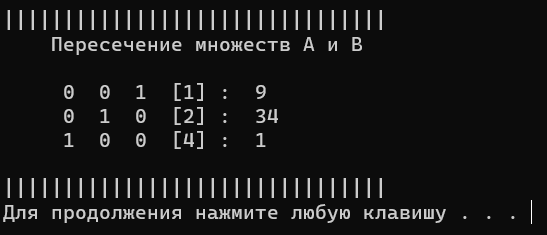
\includegraphics[width=0.6\textwidth]{7}
	\caption{Пересечение мультимножеств А и В}
\end{figure}
\clearpage
\begin{figure}[h!]
	\centering
	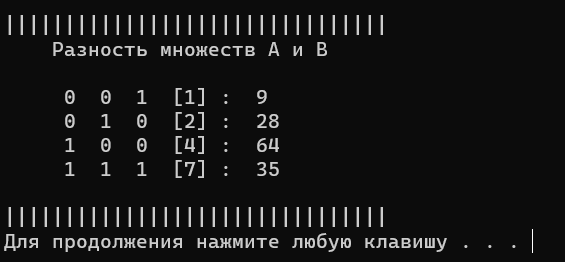
\includegraphics[width=0.8\textwidth]{8}
	\caption{Разность мультимножеств A и B}
	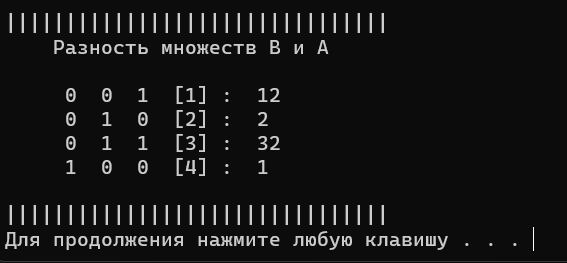
\includegraphics[width=0.8\textwidth]{9}
	\caption{Разность мультимножеств В и А}
		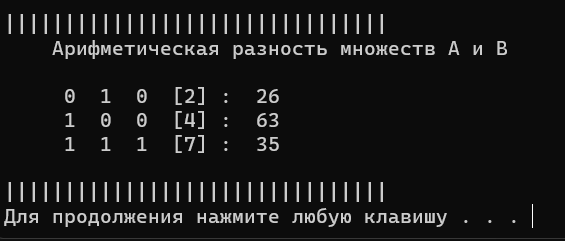
\includegraphics[width=0.8\textwidth]{10}
	\caption{Арифметическая разность мультимножеств A и B}
\end{figure}
\clearpage
\begin{figure}[h!]
	\centering
	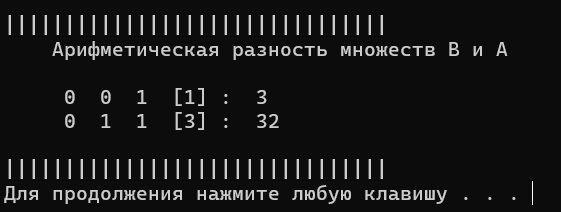
\includegraphics[width=0.8\textwidth]{11}
	\caption{Арифметическая разность мультимножеств В и А}
	
	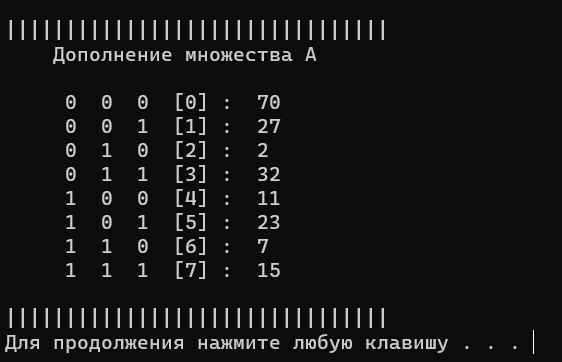
\includegraphics[width=0.8\textwidth]{12}
	\caption{Дополние мультимножества А}
	
	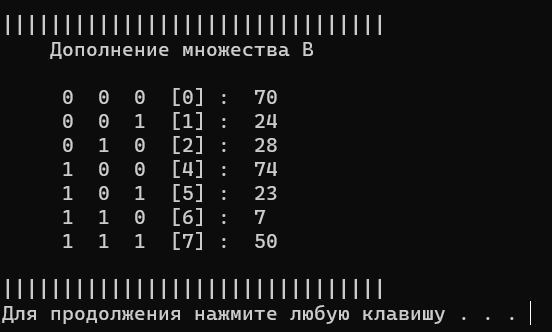
\includegraphics[width=0.8\textwidth]{13}
	\caption{Дополнение мультимножества В}
\end{figure}
\clearpage
\begin{figure}[h!]
	\centering
	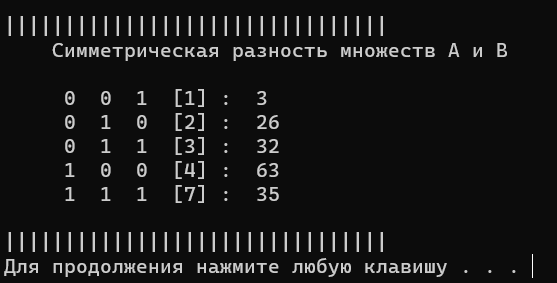
\includegraphics[width=0.7\textwidth]{14}
	\caption{Симметрическая разность мультимножеств A и B}
		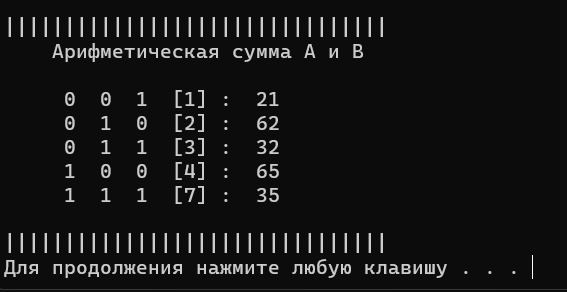
\includegraphics[width=0.7\textwidth]{15}
	\caption{Симметрическая сумма мультимножеств A и B}
		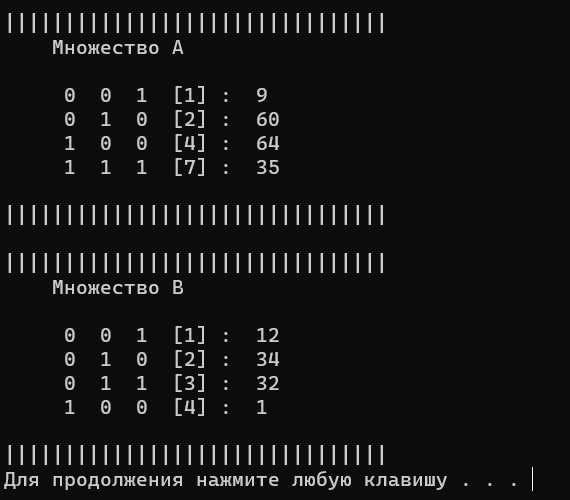
\includegraphics[width=0.7\textwidth]{17}
	\caption{Вывод на экран мультимножеств А и В}
\end{figure}
\clearpage
%\begin{figure}[h!]
%	\centering
%	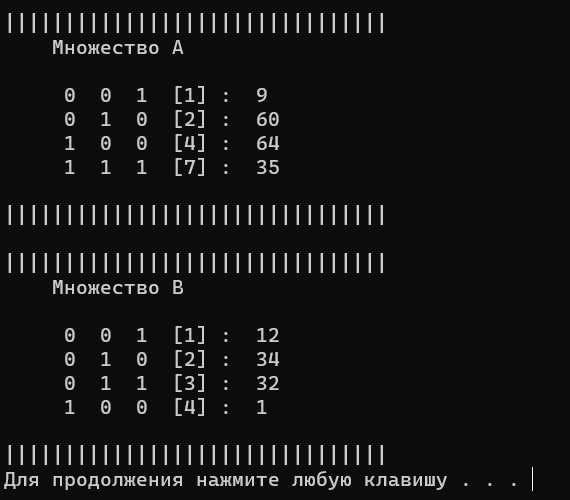
\includegraphics[width=0.8\textwidth]{17}
%	\caption{Вывод на экран мультимножеств А и В}
%\end{figure}
%\clearpage
\begin{figure}[h!]
	\centering
	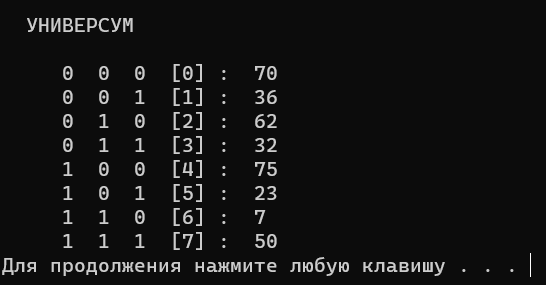
\includegraphics[width=0.8\textwidth]{18}
	\caption{Вывод на экран универсума}
\end{figure}



\newpage
\section* {Заключение}
\addcontentsline{toc}{section}{Заключение}
\par В результате выполнения лабораторной работы №1 были реализованы: программа генерации основе бинарного кода Грея для заполнения универсума заданной пользователем разрядности, мультимножества и операции над ними: объединение, пересечение, разность, арифметическая разность, дополнение, симметрическая разность, арифметическая сумма, арифметическое произведение. 
\par Из преимуществ реализованной программы, я считаю, что за счет ООП, можно использовать в других проектах классы GrayCode и Multi. Например, класс GrayCode можно использовать как генератор ланшафта, а точнее гор: уникальные элементы можно использовать как сетку, то есть квадраты которые пронумерованы попорядку, а кратность будет точкой над общим уровнем. Тогда при помощи других классов, которые будут работать с этой информацией, и както сглаживать например, а другие обрисовавать данный ландшафт, то получится, как я сяитаю, неплохая 3D модель гор. 
\par Из недостатков я считаю, что при достаточно больших разрядностях универсума и мультимножеств будет значительное занимаение памяти, а также вывод на экран универсума и мультимножеств будет достаточно долгим. Для таких случаев стоит ограничение разрядности (оно равно 10). Также если выбрать большое количество элементов мультимножества и выбрать ручной ввод, то придется очень долго вводить по одному элементу   
\par За счет такой реализации программы, можно без труда расширять классы GrayCode и Multi, а также совмещать с другими классами. В данном классе можно реализовать операции деления, возведения в степень, НОК, НОД и тд. 
\par На работу было порачено примерно 15 часов. Работа была выполнена в среде разработки Visual Studio 2022 на языке c++.

\newpage
\section* {Источники}
\addcontentsline{toc}{section}{Источники}
\begin{quote}
	1. Дискретная математика для программистов. 3-е издание. Новиков Ф.А.
	СПБ:.Питер,2009.
\end{quote}
\end{document}